\documentclass[a4paper]{article}        % Standaard een kolom layout
\usepackage[english]{babel}             % Stel woordafbrekingen en referentienamen in
\usepackage{graphicx}                   % Afbeeldingen weergeven
\usepackage{float}                      % Figuren op plaats waar ze gedefinieerd staan: [H]
\usepackage{lmodern}                     % Lettertype instellen op Helvetica
\usepackage[T1]{fontenc}
\usepackage[hidelinks]{hyperref}        % Referenties aanklikbaar in PDF, geen kaders rond weergeven
\usepackage{siunitx}                    % SI unit symbolen
\usepackage{amsmath}                    % Matrices en vergelijkingen
\usepackage{subcaption}                 % Subfiguren
\usepackage[parfill]{parskip}			% Niet inspringen aan begin alinea
\usepackage{epstopdf}

\title{Hardware Design Project\\ Designing a drone positioning sensor}
\author{Laurens Bogaert\\Thomas Deckmyn\\Zeger Van de Vannet}
\date{\today}

\begin{document}
\maketitle

% Inhoudstafel
\newpage
  \tableofcontents
\newpage

\section{Introduction}

The goal for this project is to make it possible to accurately localize drones indoor. This is for example needed if we want to make sure that the drone can fly autonomously. GPS could be used outdoor but even then is GPS not ideal since it isn't accurate enough (approximately $\SI{3}{\meter}$ accuracy in the azimuth plane and it yields even worse results in terms of determining the height of the drone). \\
That is why we will use UWB signals and thus send short pulses to determine the distances to several known anchor points. Next to this UWB antenna we need an algorithm which can determine the position of the drone accurate enough. \\
A final part of this project consists of making a board on which we can implement the algorithms.

\section{Antenna Design}
	
	For the indoor localisation of the drones we use the TIME DOMAIN\texttrademark PulsOn 400 UWB module in cooperation with a microcontroller to run the Unscented Kalman Filter algorithm. The UWB modules are already equipped with a TIME DOMAIN\texttrademark Broadspec UWB Antenna, a dipole that is omnidirectional in the azimuth plane. We will use the specifications of this antenna as design parameters for our own UWB antenna. The critical design parameters are listed below. 

	\begin{itemize}
		\item Radiate in the $\SI{3.1}{\giga\hertz}$ - $\SI{5.3}{\giga\hertz}$ band
		\item Nominal gain $\approx \SI{3}{\decibel}$
		\item Linear phase characteristic
		\item Efficiency $\approx$ 90\%	

	\end{itemize}

	\subsection{Antenna Topology and Design}
	\label{subsec:ant_design}

	At first we experiment with a few conventional UWB topologies like a bow tie and a barbell shape (see Figure \ref{fig:topologies}). After optimisation and simulation in ADS, we conclude that the simulated S-parameters and gain are not compliant with the design parameters above. Obtaining a linear phase characteristic with these topologies proves to be very hard as well.  

		\begin{figure}[H]
		\begin{subfigure}{0.5\textwidth}
			\centering
			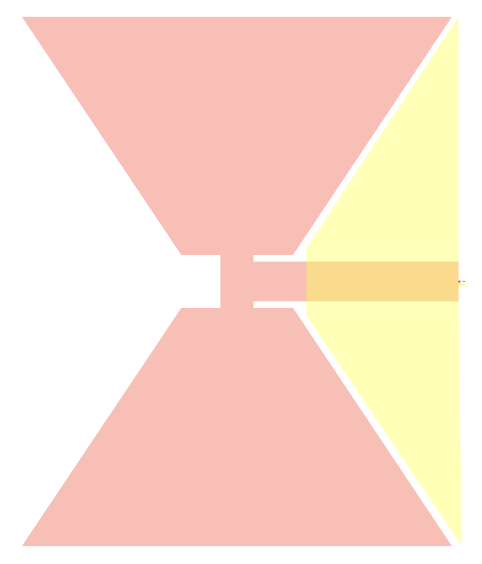
\includegraphics[width=0.5\textwidth,height=85px]{images/antenna/bow_tie.png}
			\caption{Bow Tie Topology}
		\end{subfigure}
		\begin{subfigure}{0.5\textwidth}
			\centering
			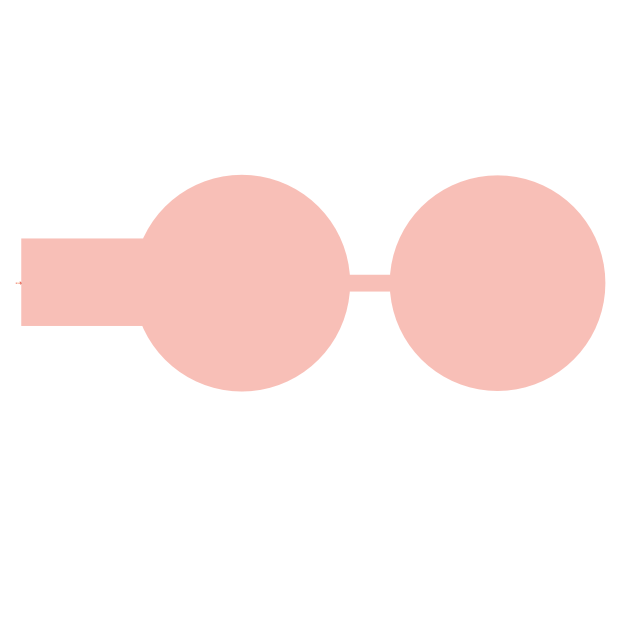
\includegraphics[width=0.5\textwidth]{images/antenna/bar_bell.png}
			\caption{Barbell Topology}
		\end{subfigure}
		\caption{UWB Antenna Topologies}
		\label{fig:topologies}
		\end{figure} 

	The substrate material that is being used to design the antenna is \textit{Black Foam} with a low relative permittivity $\epsilon_r = 1.495$. Because of this we encounter a practical problem with respect to the dimension of the antenna, i.e. if the antenna needs to be constructed with this substrate its dimension will be too large to mount on the drone. Thus for the remaining part of the design process we opt for an \textit{Aromated Polyurethane} substrate with a higher $\epsilon_r = 2.55$, which allows us to work with smaller dimensions while radiating in the same frequency band. 

	After experimenting with the exotic topologies mentioned above, we redo the design starting from a rectangular microstrip patch antenna. The length of the patch determines the resonance frequency of the device, while the width has an influence on the radiated power. A wider patch means less resonance resistance, hence more bandwidth and a higher efficiency. 
	We want the resonance frequency of the patch to be in the predefined frequency band $\SI{3.1}{\giga\hertz}$ - $\SI{5.3}{\giga\hertz}$ and thus choose $f_0 = \SI{4.2}{\giga\hertz}$. Using equation (\ref{eq:width_patch}) we calculate the desired width of the patch.
	\begin{equation} 
	L = \frac{c}{2 f_r \sqrt{\epsilon_r}}
	\label{eq:width_patch}
	\end{equation}

	The bandwidth of the antenna needs to be very wide, thus, as explained above, we would be tempted to increase the width of the patch to obtain a bigger bandwidth. Again, we are limited by the dimensions of the drone, because it needs to be fitted onto the drone and we don't want the antenna to interfere too much with the aerodynamics. To increase the bandwidth we apply another technique, i.e. adding stairs to the rectangular patch and optimizing their dimensions to obtain the desired bandwidth. Also, we introduce a partial ground plane, of which we again optimize the dimensions, to realize an approximately flat $S_{11}$ and a linear phase characteristic in the wanted frequency band. The final antenna lay-out is shown in Figure \ref{fig:patch_stairs} and the optimized dimensions are given in Table.

	\begin{figure}[H]
	\centering
		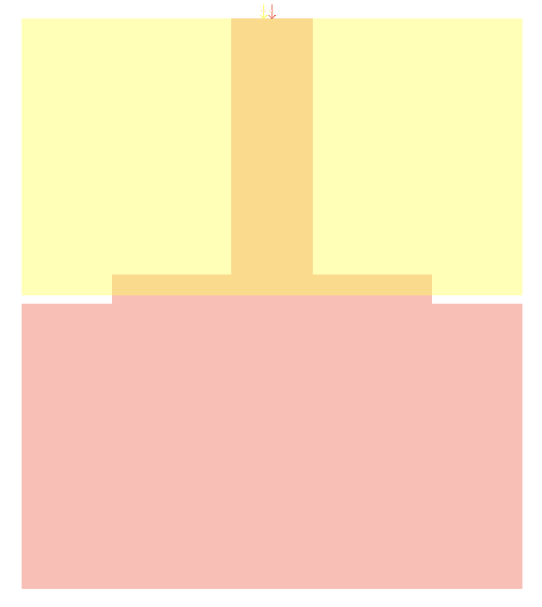
\includegraphics[width=0.5\textwidth]{images/antenna/patch_stairs.png}
		\caption{Rectangular patch antenna with added stairs and partial ground plane}
		\label{fig:patch_stairs}
	\end{figure}

	\begin{table}[H]
	\centering
	\begin{tabular}{|c|c|}
		\hline
		\multicolumn{2}{|c|}{\textbf{Antenna}} \\ \hline
		L & $\SI{20.5}{\milli\meter}$ \\ \hline
		W & $\SI{36}{\milli\meter}$ \\ \hline
		$W_{stair}$ & $\SI{8.6}{\milli\meter}$ \\ \hline
		$H_{stair}$ & $\SI{2.1}{\milli\meter}$ \\ \hline
		\multicolumn{2}{|c|}{\textbf{Ground Plane}} \\ \hline
		L & $\SI{19.2}{\milli\meter}$ \\ \hline
		W & $\SI{36}{\milli\meter}$ \\ \hline 
	\end{tabular}
	\caption{Optimized dimensions for antenna and partial ground plane}
	\label{tab:dimensions}
	\end{table}

	\begin{figure}[H]
	\centering
	\begin{subfigure}[b]{0.52\textwidth}
                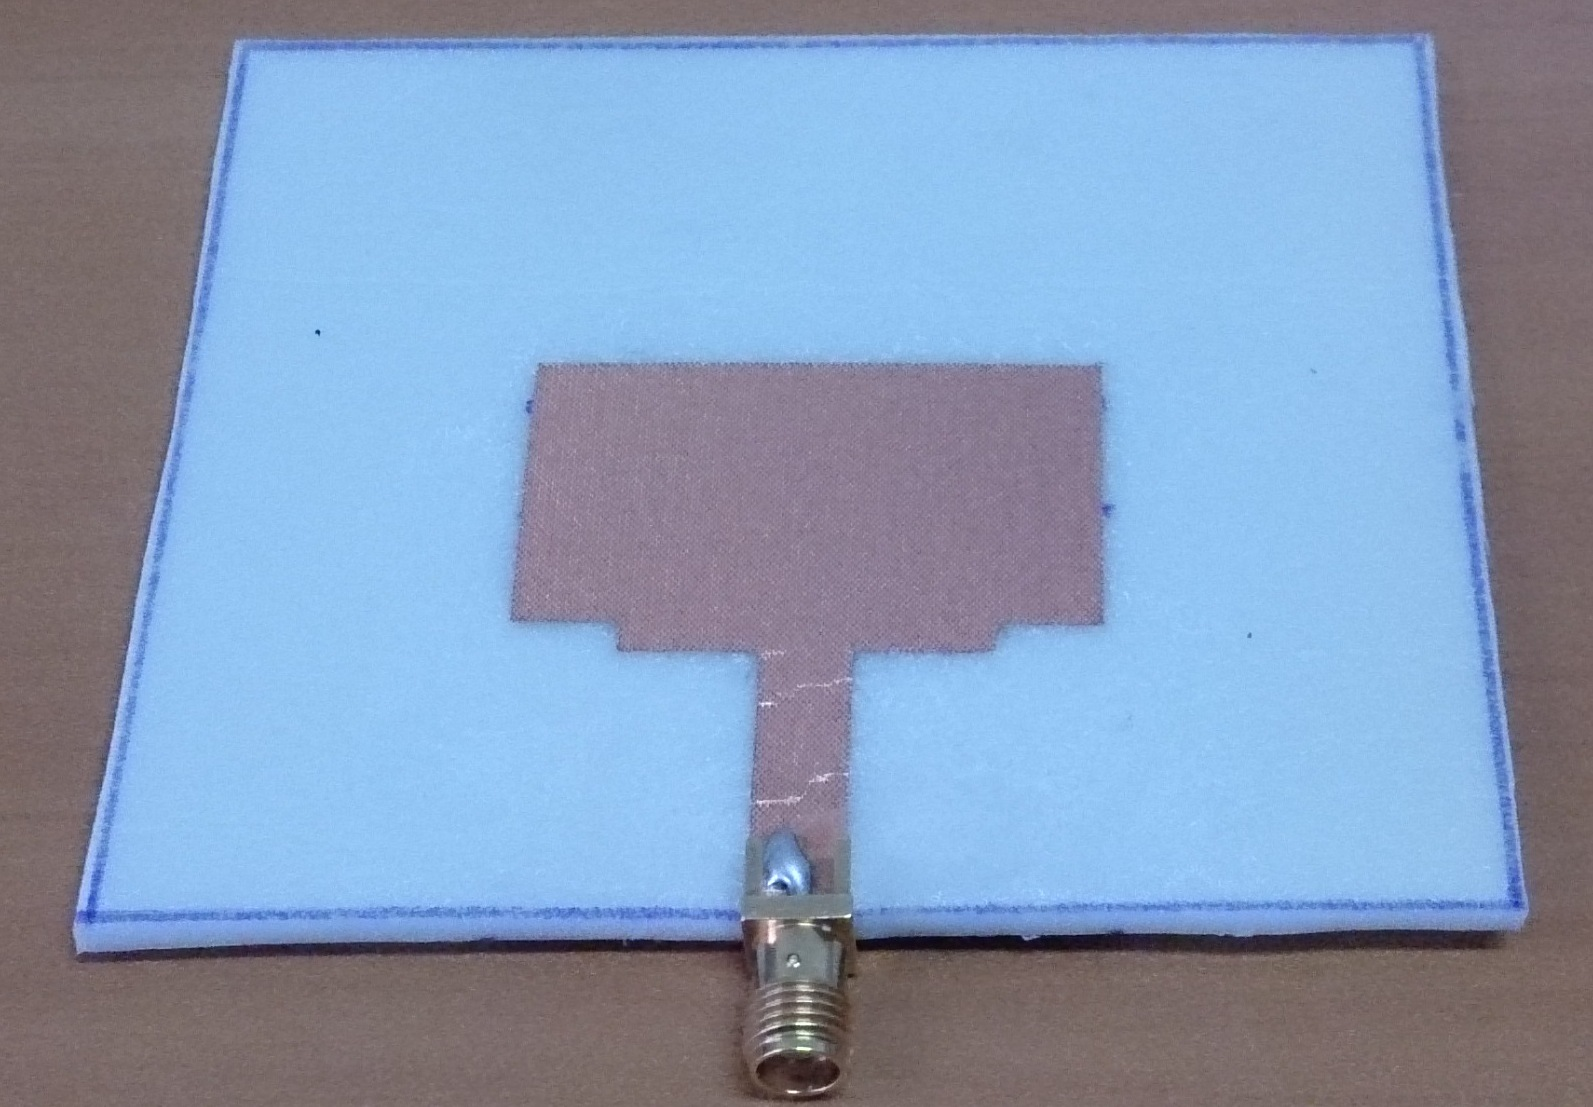
\includegraphics[width=\textwidth]{images/patch_proto_front}
                \caption{Front side prototype antenna}
                \label{fig:front_prototype}
        \end{subfigure}%
  ~      
        \begin{subfigure}[b]{0.5\textwidth}
                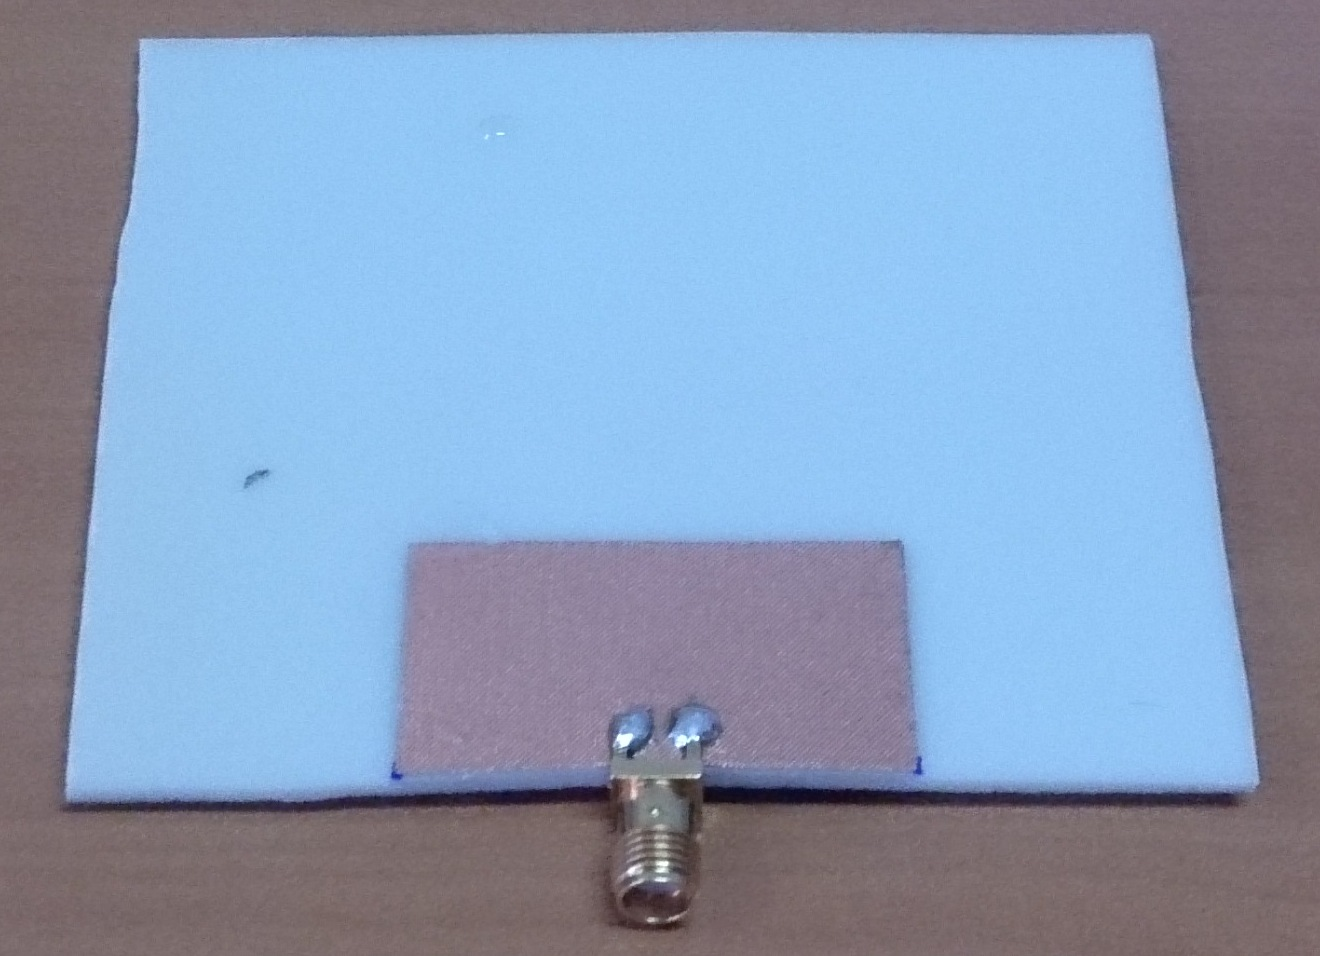
\includegraphics[width=\textwidth]{images/patch_proto_back}
                \caption{Back side prototype antenna}
                \label{fig:back_prototype}
        \end{subfigure}
	\end{figure}

	\subsection{Simulation}
		While designing the antenna, simulations in ADS are used to confirm that the antenna's characteristics are as desired. In this section we will discuss the simulation results of the final design, as explained in the previous section \ref{subsec:ant_design}. 

		\begin{figure}[H]
		\begin{subfigure}{0.5\textwidth}
		\centering
			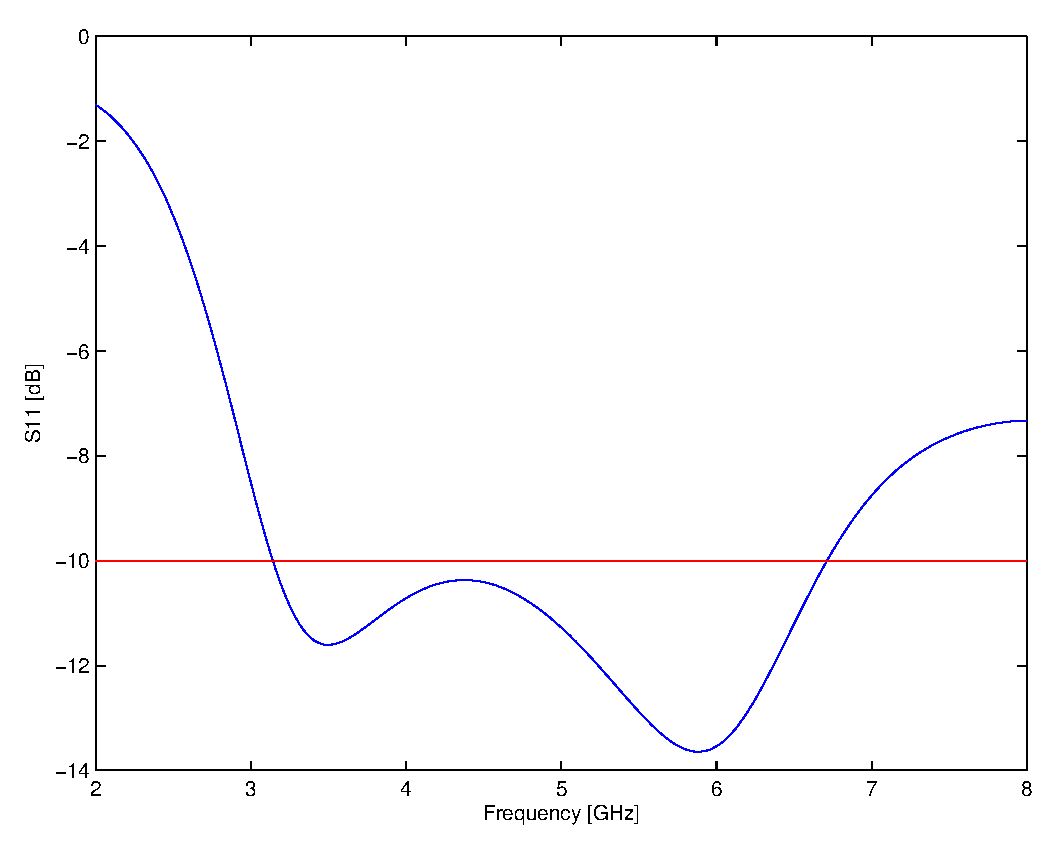
\includegraphics[width=\textwidth]{images/S11_ADS_sim.eps}
			\caption{Simulated $S_{11}$}
		\end{subfigure}
		\begin{subfigure}{0.5\textwidth}
		\centering
			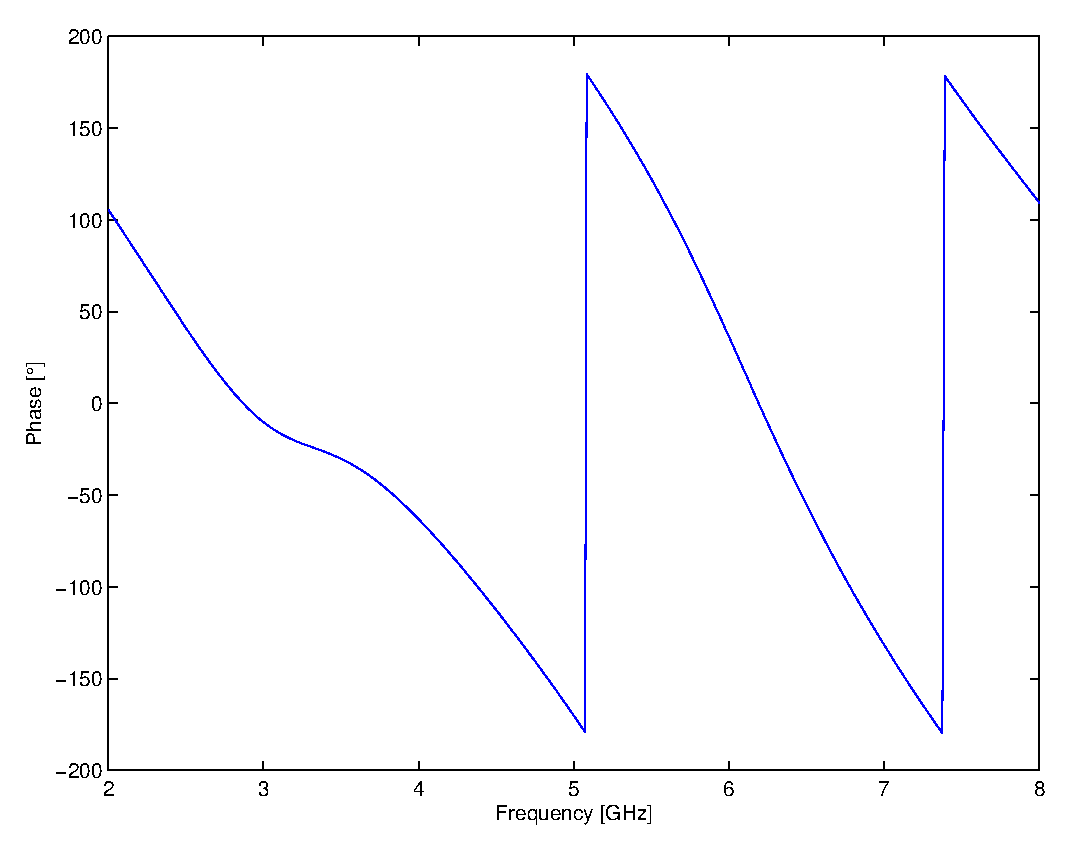
\includegraphics[width=\textwidth]{images/fase_respons_ADS_sim.eps}
			\caption{Simulated phase response}
		\end{subfigure}
		\caption{Simulated characteristics for designed UWB antenna}
		\label{fig:S11_phase_design}
		\end{figure}

		Figure \ref{fig:S11_phase_design} shows that the $S_{11}$-parameter is below $\SI{-10}{\decibel}$, and relatively flat, in the desired frequency band. The phase characteristic proves to be approximately linear as well, which is in line with the design parameters. The gain is ca. $\SI{3}{\decibel}$ and the antenna efficiency is between 50\% and 96\% in the lower half of the frequency band, according to the simulation. 

	\subsection{Measurements}
		After the positive simulation results, we continue with the construction of the designed antenna. Due to a small misalignment between partial ground plane and antenna we need to construct a second version of the UWB antenna to obtain optimal results. Between these two versions, some minor adjustments are made to the design to further improve flatness of the $S_{11}$ and linearity of the phase. The measured reflection coefficient of the two versions\footnote{The initial measurements of the S-parameters of both versions suffered from noise due to common-mode current, which was solved by addition of a ferrite clamp.} of the antenna is compared to the reference antenna and to the respective simulation in Figure \ref{fig:antenna_comp}. 

		\begin{figure}[H]
			\centering
			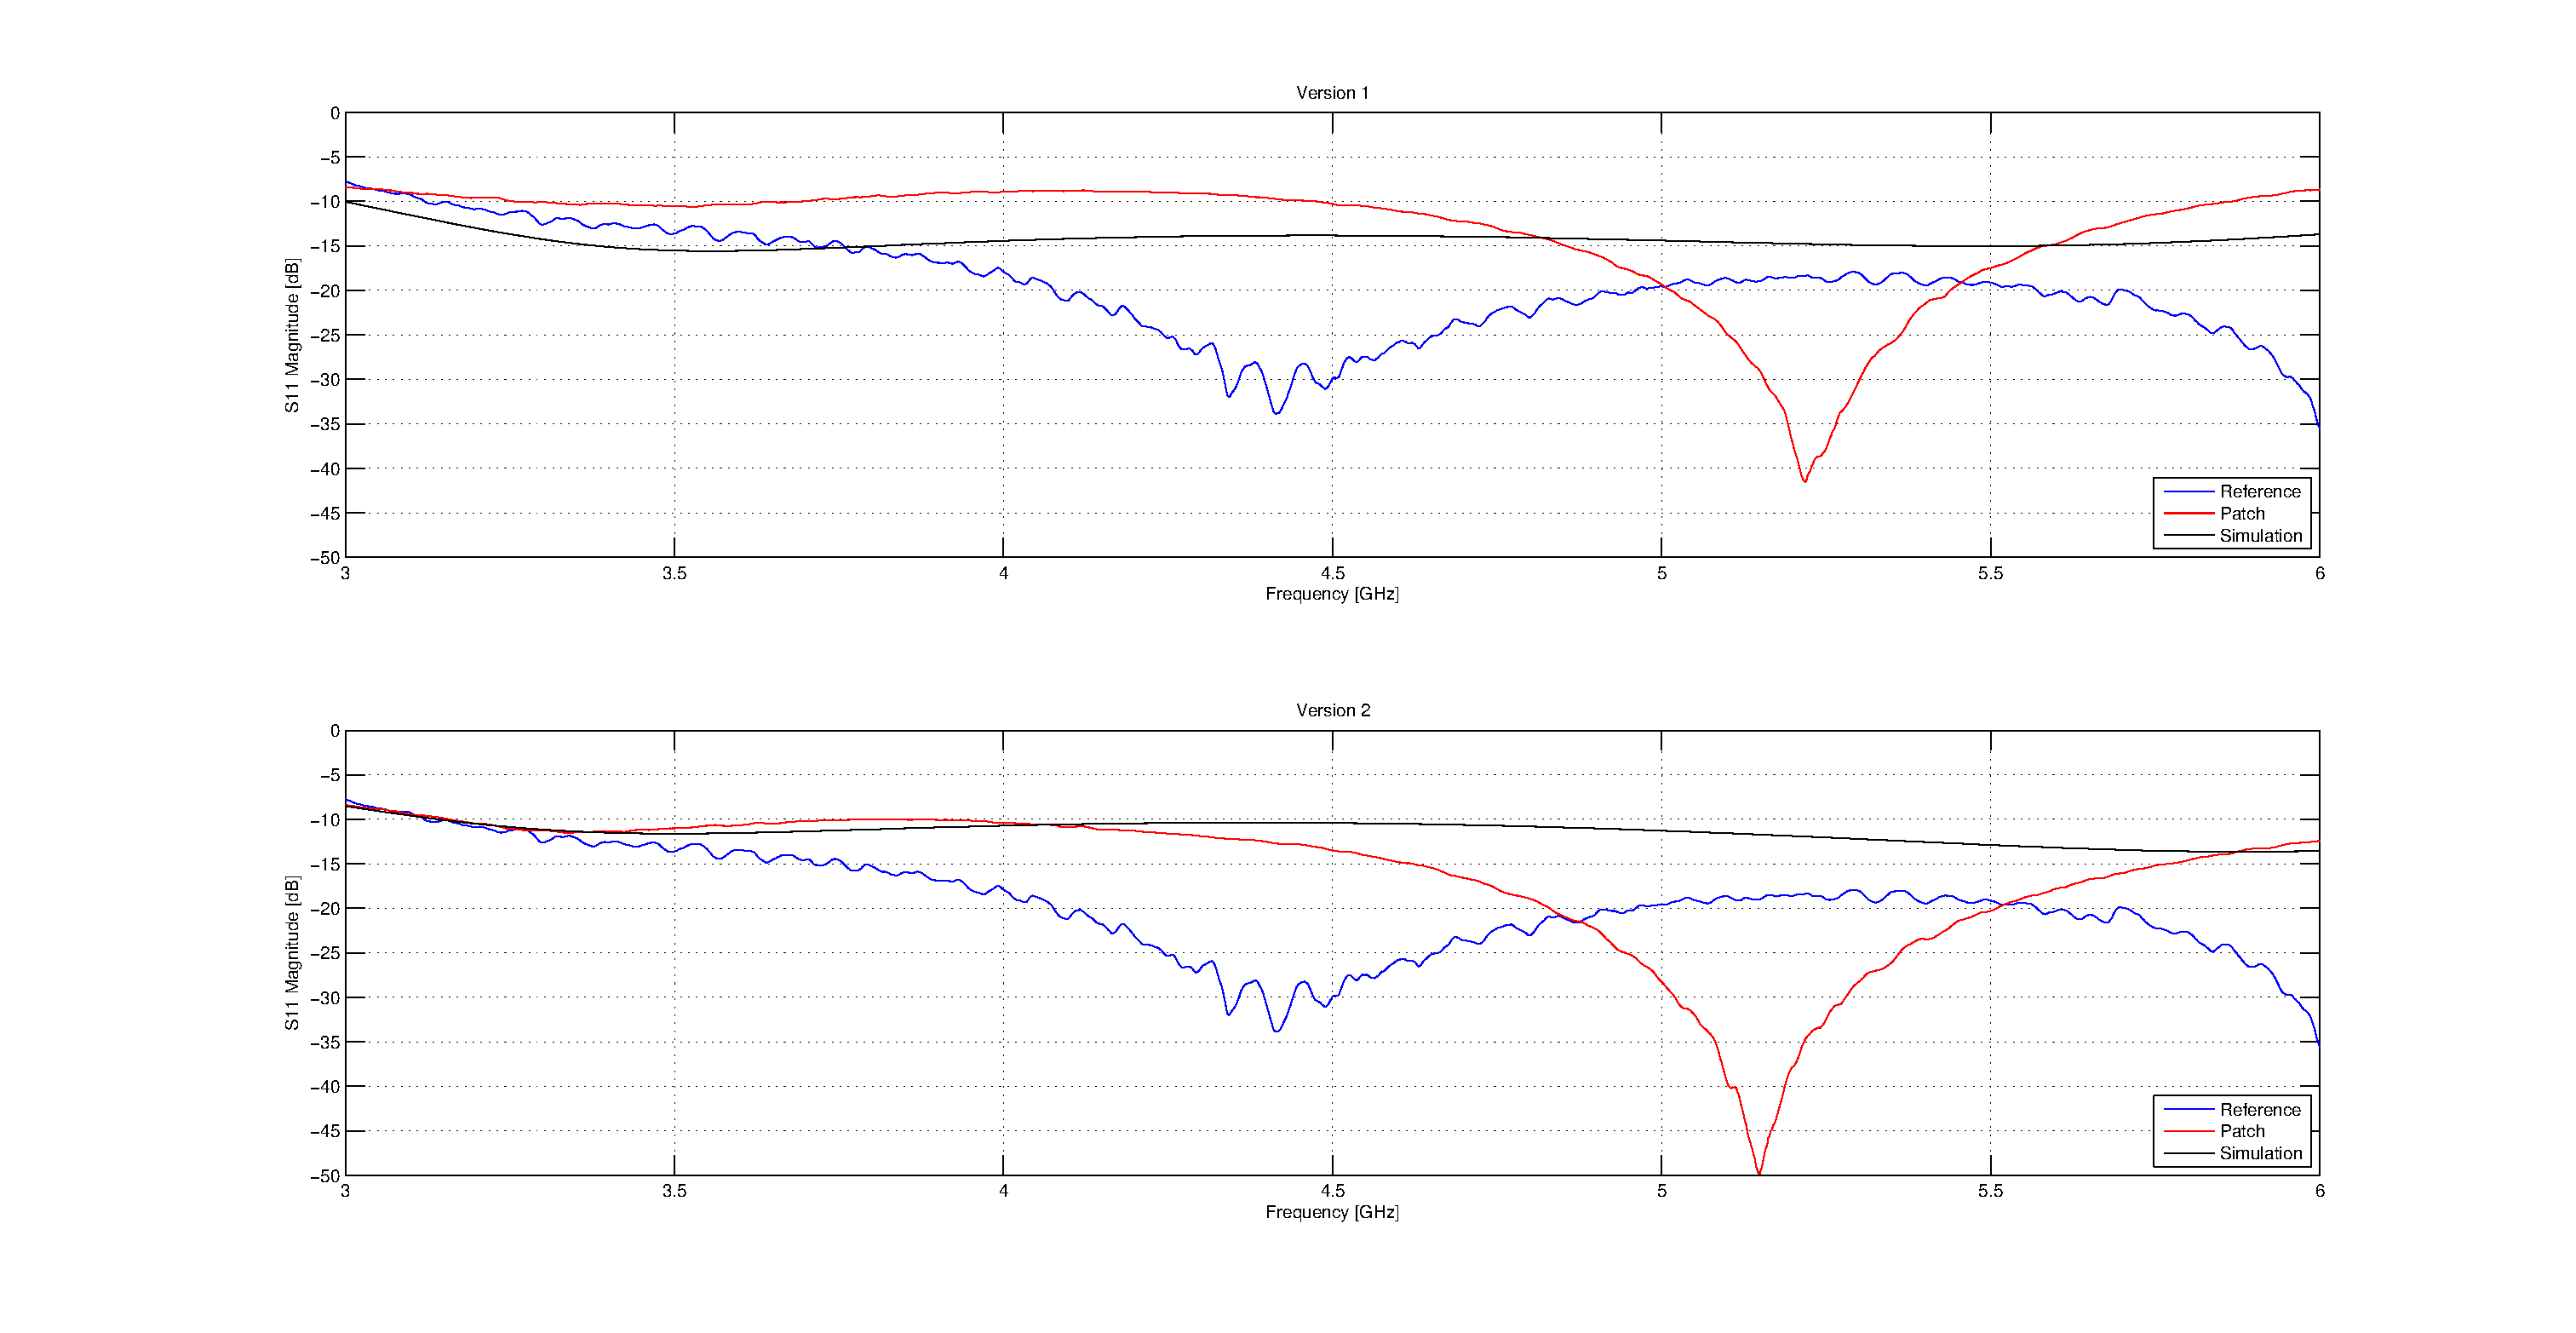
\includegraphics[width=\textwidth]{images/antenna/antenna_comparison}
			\caption{Version 1 and 2 of constructed antenna compared to simulation and reference}
			\label{fig:antenna_comp}
		\end{figure}

		As seen on Figure \ref{fig:antenna_comp}, the first version of the antenna doesn't meet the pre-imposed design criteria, i.e. the $S_{11}$ is not smaller than $\SI{-10}{\decibel}$ over the entire frequency range.
		The $S_{11}$ characteristic is improved by the better alignment in version 2 and the minor adjustments to the design.

		



\section{Location Algorithm}
	A first algorithm that can be used to determine the position of the drone is the \textit{Least Mean Square} algorithm. We will elaborate on this first and then compare the performance to the Unscented Kalman Filter, which will be used in the final system. 

	\subsection{Least Mean Square}
	\label{subsec:LMS}

		The LMS algorithm uses the distances between the drone and a number of well-known anchor points to determine the position. The UWB antenna mounted on the drone broadcasts a very short pulse to the anchors, which will return the same pulse when it is received. The board on the drone measures the time between sending the pulse and receiving it back. Because the propagation speed of the pulse through air and the time it takes to process the pulse at the anchors are known, the distance to the anchor points can be determined as follows:

		\begin{equation}
		\centering
			t_{roundtrip} = 2t_{propagation} + t_{process}
		\end{equation} 

		Because the time to process the pulse at the anchor is known, we can calculate the time it takes to bridge the distance between the drone and the anchor point. With $c$ the speed of light ($\SI{3e8}{\meter\per\second}$) this results in an expression for the distance to anchor point $i$:

		\begin{equation}
		\centering
			d_i = c*t_{propagation}
		\end{equation}

		With $\vec{\textbf{x}}$ denoting the position vector $\begin{bmatrix} x & y & z \end{bmatrix}$ of the drone and $\vec{\textbf{x}_i}$ the position vector $\begin{bmatrix} x_i & y_i & z_i \end{bmatrix}$ of the $i^{th}$ anchor point, this distance can also be expressed as follows:

		\begin{align*}
		\centering
			d_i^2 &= (\vec{\textbf{x}} - \vec{\textbf{x}_i})(\vec{\textbf{x}} - \vec{\textbf{x}_i})^T \\
			&= x^2 - 2x_ix + x_i^2 + y^2 - 2y_iy + y_i^2 + z^2 - 2z_iz + z_i^2
		\end{align*}

		This equation is not linear in x, y and z and therefore it is hard to extract the position vector. With $d_N$ the distance to the $N^{th}$ anchor, the equation can be linearised as follows:

		\begin{align*}
		\centering
			d_i^2 - d_N^2 &= x^2 - 2x_ix + x_i^2 + y^2 - 2y_iy + y_i^2 + z^2 - 2z_iz + z_i^2 - d_N^2 \\
				&= 2x(x_N - x_i) + 2y(y_N - y_i) + 2z(z_N- z_i)+ (x_i^2 - x_N^2) + (y_i^2 - y_N^2)  + (z_i^2 - z_N^2) 
		\end{align*}

		This yields a matrix representation of the form $\textbf{A}\vec{\textbf{x}} = \textbf{B}$ which can be solved for the position vector $\vec{\textbf{x}}$.


	% subsection LMS (end)
	\subsection{Kalman Filtering}
	The second algorithm that is implemented is the Kalman Filter. This algorithm makes use of ``sensor'' fusion which in principle means that we try to combine data from several sensors to track the drone more accurately.
	Examples from sensors that we can use to improve the result are an accelerometer, a gyroscope, an altitude meter, etc.\\
	The iterative process of a Kalman filter consists of 2 distinct steps. First of all we will try to predict the next location by using results of the past (i.e. Kalman filtering is a method with a memory). 
	The second step of Kalman filtering consists of using the real measured data (distances and possibly also extra data) to update the memory of the filter by changing the matrices in the Kalman filter system.\\
	However, the matrix computations used in the implementation of the Kalman filter are based on Gaussian distributions. Hence, in real life (when we don't have Gaussian distributed data) we won't get as good performances as we get when simulating the Kalman filter.
	%CONCEPTUAL SOLUTION FOR THIS PROBLEM?
	
\subsection{Comparison between LMS and Kalman}

To compare both algorithms we generate a Gaussian movement and calculate the distance to each of the anchors in a noiseless channel. Then we generate the input distances for the algorithm by adding Gaussian noise to the ideal distances.
When we display the generated movement on a plot which also consists of the output locations of the Kalman filter and LMS algorithm we get figure \ref{fig:paths}.
We notice on this figure that the path is followed quite accurately, but to make a real comparison between the 2 algorithms we will have to zoom in on a part of the followed route. This is what is done in figure \ref{fig:paths_zoom}.	

			\begin{figure}[H]
				\centering
				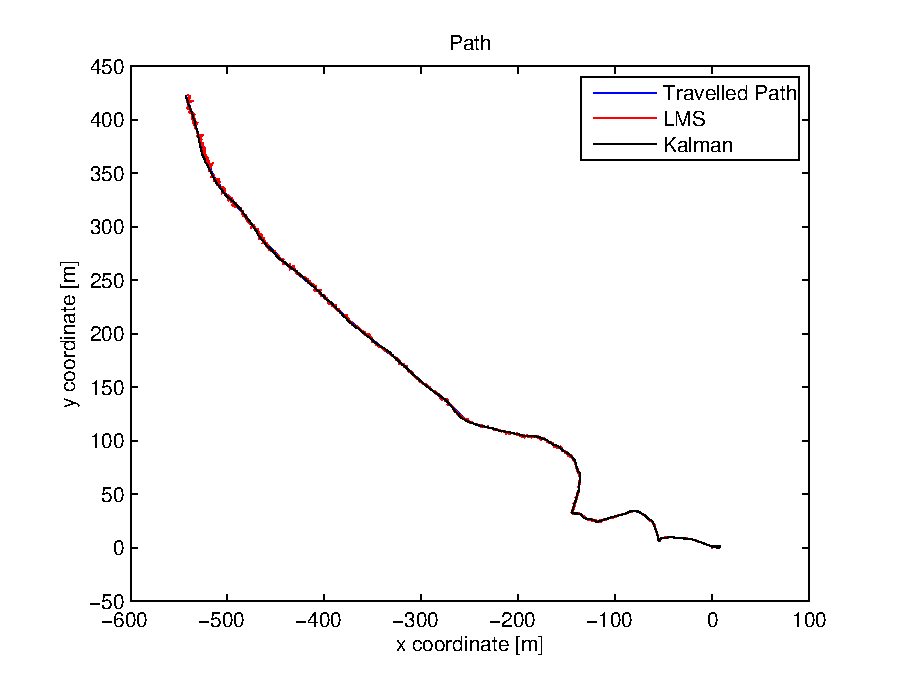
\includegraphics[width=\textwidth]{images/tracking_algorithms.eps}
				\caption{Travelled paths according to the different algorithms}
				\label{fig:paths}
			\end{figure}

		
			
			\begin{figure}[H]
				\centering
				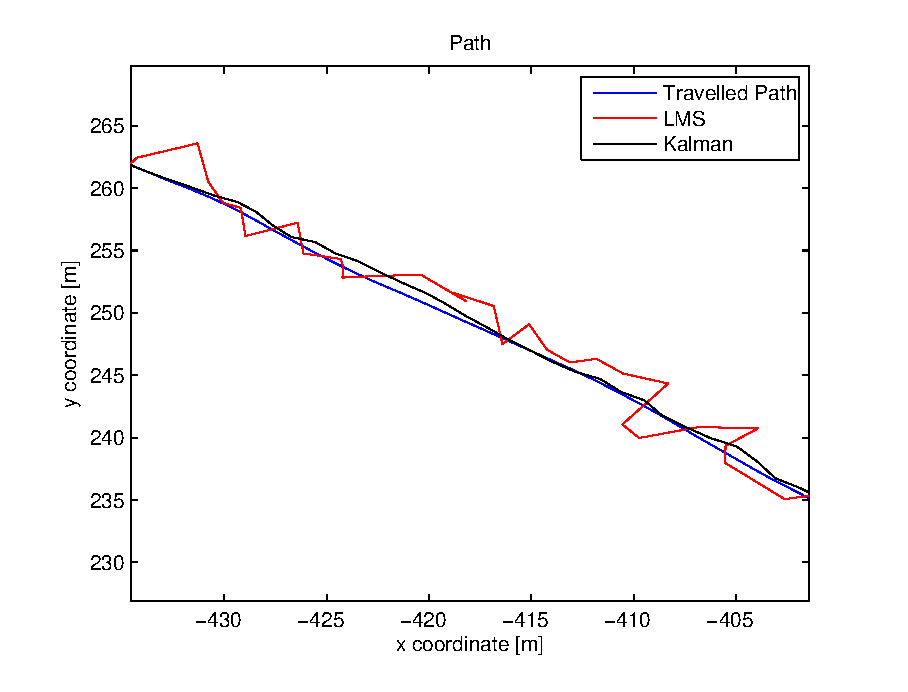
\includegraphics[width=\textwidth]{images/tracking_algorithms_zoom.eps}
				\caption{Travelled paths according to the different algorithms (zoom)}
				\label{fig:paths_zoom}
			\end{figure}

On figure \ref{fig:paths_zoom} it can be seen that LMS is somewhat worse than the Kalman Filter. Next to this, it has to be mentioned that the Kalman path is way smoother than the path followed according to LMS. This is because the Kalman uses a memory and states that big jumps in the followed direction are very unlikely and thus Kalman locally follows a path that resembles a straight line. Hence, Kalman will only be useful if we use our algorithm to try to track a drone which doesn't change its course too abruptly.
Now, we want to quantize the error made by adopting both algorithms. We choose as a distortion measure the mean squared error per dimension and let Matlab plot the cumulative distribution function of this mean squared error (figure \ref{fig:cdf}). This cdf learns us that the LMS indeed yields worse performances than the Kalman when a Gaussian-based path is followed and we don't introduce too much measure noise.
			
			\begin{figure}[H]
				\centering
				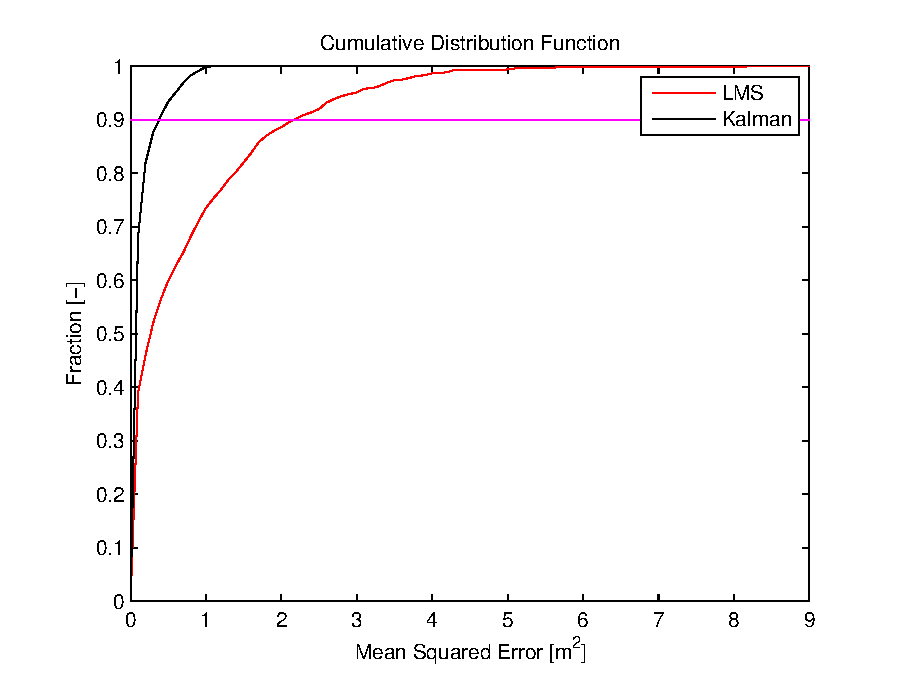
\includegraphics[width=\textwidth]{images/cdf_algorithms.eps}
				\caption{Cumulative distribution function for the different algorithms}
				\label{fig:cdf}
			\end{figure}

The mean squared error per dimension that was mentioned before is computed as follows:

\begin{equation}
MSE = \dfrac{1}{3}((x_{real}-x_{est})^2+(y_{real}-y_{est})^2+(z_{real}-z_{est})^2)
\end{equation}

On figure \ref{fig:cdf}, a purple line is included which gives us the 90th percentile:

\begin{table}[H]
\begin{center}
\begin{tabular}{ | r | l | }
    \hline
     & MSE [$m^2$] \\ \hline
    LMS & $\SI{1.95}{\square\meter}$ \\ \hline
    Kalman & $\SI{0.43}{\square\meter}$ \\
    \hline
\end{tabular}
\end{center}
\caption{Mean Squared Error: a comparison}
\label{table:MSE}
\end{table}

\section{PCB Design}
  In order to process the measurements and determine the position of the drone, a microcontroller is attached to one of the RCM modules.
  These modules can be used both for ranging measurements, as well as for wireless communication. The module with the microcontroller is attached to the drone and several other RCM modules are placed in the room or building to serve as anchor points. An additional RCM is connected to a computer which acts as a central control unit and also allows to visualise the position of the drone in real time.

  As microcontroller we choose one from the STM32F4XX-series. These are powerful 32 bit ARM processors, which are sufficiently fast to process the data.
  To attach it to the ranging module, we design a PCB to hold the processor and its required decoupling. Communication with the module is provided by a USART interface.
  A voltage regulator yields a stable $\SI{3.3}{\volt}$ from different sources: either from an external battery or from the drone itself. Switching between both supplies can be done by moving a jumper.

  To improve the results from the Kalman filter, an accelerometer is also added to the design, which provides acceleration data in three dimensions. Communication with the accelerometer is done over the I2C interface.

  To protect the microcontroller from ESD damage, we add Zener diodes to every IO pin, which will safely dispose of the harmful power injected into the system.

  
\end{document}

